% ---
% Reemplaza líneas 1761-1802 de Docs/Technical_Report.tex
% Decisiones: D-028, D-032, H-033, H-038
% ---

\subsubsection{\textit{Geometric difference}}

La \textit{geometric difference} fue formalizada por Huang et al. \cite{huang2021power}
para evaluar si un kernel cuántico $K_Q$ induce sobre los datos una geometría que un kernel
clásico $K_C$ dado no puede reproducir.
Dados $K_Q, K_C \in \mathbb{R}^{N \times N}$ normalizados a traza común $\operatorname{Tr}(K_Q) = \operatorname{Tr}(K_C) = N$,
la \textit{geometric difference} sin regularizar es:
\begin{equation}
  g_{CQ} = g(K_C \parallel K_Q) = \sqrt{\left\| \sqrt{K_Q}\;K_C^{-1}\;\sqrt{K_Q} \right\|_\infty},
  \label{eq:geometric_diff}
\end{equation}
donde $\|\cdot\|_\infty$ denota la norma espectral (el autovalor máximo de la matriz simétrica)
y $\sqrt{K}$ es la raíz cuadrada matricial simétrica positiva obtenida por descomposición
espectral:
\begin{equation}
  K = V \Lambda V^\top \implies \sqrt{K} = V \Lambda^{1/2} V^\top,
  \label{eq:spectral_sqrt}
\end{equation}
con truncamiento a cero de posibles autovalores residuales negativos por precisión de punto
flotante. En la ecuación~\eqref{eq:geometric_diff}, el kernel cuántico $K_Q$ figura en los
factores externos mientras que el kernel clásico $K_C$ es la matriz invertida.
Con kernels de diagonal unitaria y $\operatorname{Tr}K=N$, $g_{CQ}\ge1$: basta evaluar el cociente de Rayleigh $v^\top K_Q v / v^\top K_C v$ en un vector canónico.

En conjuntos de datos reales, la evaluación directa de la ecuación~\eqref{eq:geometric_diff}
resulta numéricamente inestable debido a que las matrices de kernel clásicas suelen presentar
valores propios muy pequeños, que disparan $g_{CQ}$ y hacen que mida el condicionamiento de $K_C$ y no la codificación. Para subsanar esto, Huang et al. \cite{huang2021power} definieron
% respaldo: «When we only have a finite number N of training samples, we can use the fact that k(x, y) = φ(x)†φ(y) and the definition that Kij = k(xi, xj) to obtain» (huang2021powerSupp, p. 12)
% Equivalencias con la versión de arXiv (2011.01938): sección 6 C = Apéndice F.3; (S71) = (F19); (S72) = (F20).
la formulación regularizada mediante un parámetro de penalización $\lambda > 0$ (información suplementaria, sección~6\,C, ecs.~(S71) y~(S72)):
\begin{equation}
  g_{\text{gen}}(K_C, K_Q; \lambda) = \sqrt{\left\| \sqrt{K_Q}\sqrt{K_C}\,(K_C + \lambda I)^{-2}\,\sqrt{K_C}\sqrt{K_Q} \right\|_\infty},
  \label{eq:g_gen}
\end{equation}
junto con la cota del error de entrenamiento admisible para el predictor clásico:
\begin{equation}
  g_{\text{tra}}(K_C, K_Q; \lambda) = \lambda\,\sqrt{\left\| \sqrt{K_Q}\,(K_C + \lambda I)^{-2}\,\sqrt{K_Q} \right\|_\infty}.
  \label{eq:g_tra}
\end{equation}
Cuando $\lambda \to 0$, $g_{\text{gen}}$ recupera la distancia de la ecuación~\eqref{eq:geometric_diff}.

% respaldo: «We consider the following list of λ λ ∈{0.00001, 0.0001, 0.001, 0.01, 0.025, 0.05, 0.1},» (huang2021powerSupp, p. 20)
% Equivalencias con arXiv: sección 12 C = Apéndice L.3; (S113)–(S115) = (L9)–(L11).
Se sigue el protocolo de Huang et al. (información suplementaria, sección~12\,C,
ecs.~(S113)--(S115)): se evalúa una malla de
regularización $\lambda \in \{10^{-5}, 10^{-4}, 10^{-3}, 10^{-2}, 0.025, 0.05, 0.1\}$ y una
batería de kernels clásicos que comprende un kernel lineal sobre los datos centrados
y kernels gaussianos (RBF) con parámetro $\gamma = m / (n\,\operatorname{Var}[\mathbf{x}])$,
para multiplicadores $m \in \{0.25,\allowbreak 0.5,\allowbreak 1,\allowbreak 2,\allowbreak 4,\allowbreak 8,\allowbreak 16,\allowbreak 32,\allowbreak 64\}$, con $n = 12$ el número de
características y $\operatorname{Var}[\mathbf{x}]$ la varianza de todas las coordenadas de la submuestra.
Como análisis de sensibilidad se añaden gaussianos más estrechos, $m \in \{128, 256, 512\}$.
Para cada kernel clásico, se identifica el mayor valor de $\lambda$ admisible que satisface la
restricción de error de entrenamiento:
\begin{equation}
  g_{\text{tra}}(K_C, K_Q; \lambda) < 0.045,
  \label{eq:gtra_admissibility}
\end{equation}
y se reporta el valor mínimo alcanzable sobre toda la batería,
$g = \min_{K_C} g_{\text{gen}}(K_C, K_Q; \lambda^*(K_C))$.

El criterio de decisión teórico establecido por Huang et al. contrasta este valor frente a la
cota de dimensión de la muestra:
\begin{itemize}
  \item Si $g \ll \sqrt{N}$ (donde $\sqrt{N} = \sqrt{200} \approx 14.14$), el modelo clásico
        predice con un error comparable o menor cualquier función que el modelo cuántico pueda
        aprender, sea cual sea el etiquetado.
  \item Si $g$ es del orden de $\sqrt{N}$, existe un etiquetado para el que el modelo cuántico
        puede superar a los clásicos de la batería. Es una condición necesaria, no suficiente: la
        ventaja depende además de las etiquetas reales.
\end{itemize}

El cálculo se realiza sobre una submuestra fija de exactamente $N = 200$ lesiones estratificadas
por clase del conjunto de entrenamiento por cada subproblema (semilla 42). La
figura~\ref{fig:huang_geometria} ilustra el marco geométrico conceptual propuesto por Huang et al.

\begin{figure}[htbp]
  \centering
  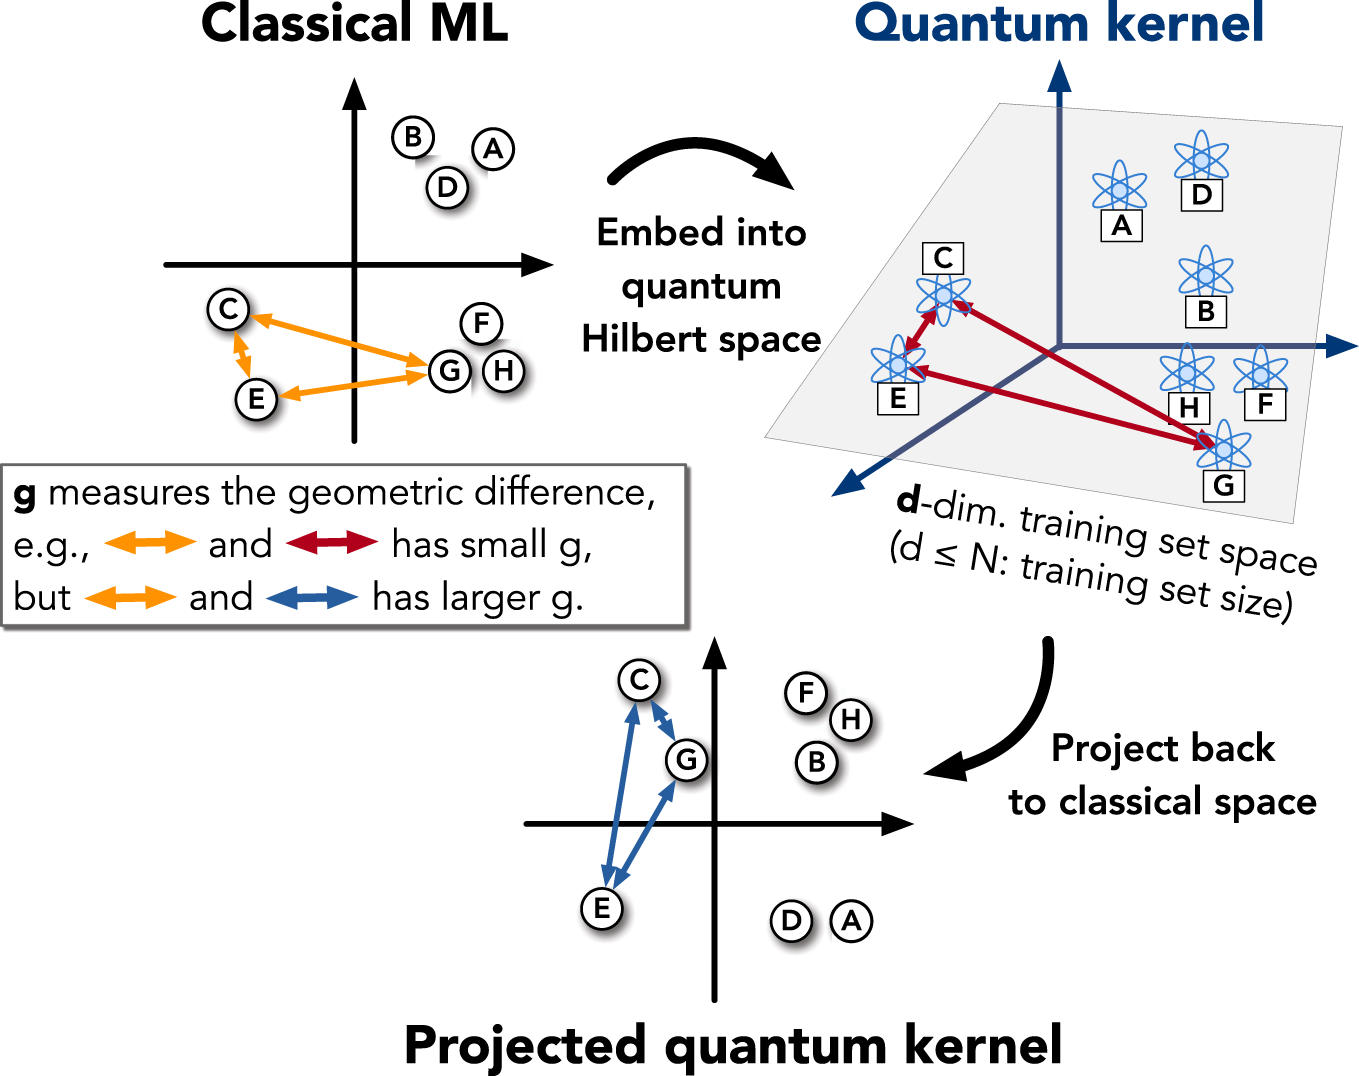
\includegraphics[width=0.7\textwidth]{Figures/Huang2021_Fig2.png}
  \caption{Geometría (función kernel) definida por modelos clásicos y cuánticos. Las letras
  representan datos y las flechas, la similitud entre ellos; la \textit{geometric difference}
  \(g\) mide cuánto difieren esas similitudes entre modelos, y \(d\) es la dimensión efectiva
  del conjunto de entrenamiento en el espacio de Hilbert. Reproducida de Huang et al. (2021),
  \textit{Nat. Commun.} 12, 2631, bajo licencia CC BY 4.0 (\protect\url{https://creativecommons.org/licenses/by/4.0/}).}
  \label{fig:huang_geometria}
\end{figure}

\textbf{Concentración exponencial del kernel cuántico.}
Un obstáculo para escalar de clasificadores cuánticos basados en producto interno
es el fenómeno de concentración, advertido por Huang et al. (``\textit{all inputs are too far apart}'')
y formalizado por Thanasilp et al. \cite{Thanasilp2024}. A medida que el número de qubits $n$
crece, las fidelidades cuánticas fuera de la diagonal
$|\langle\phi(\mathbf{x})|\phi(\mathbf{x}')\rangle|^2$ se concentran exponencialmente en $n$ alrededor de un valor fijo, que para el kernel de fidelidad
es cercano a cero. El kernel se acerca entonces a la matriz identidad, $K_Q \approx I$: todas las
muestras parecen casi ortogonales entre sí y se pierde la noción de vecindad.
Thanasilp et al. identifican cuatro fuentes de concentración: la expresividad del \textit{embedding},
las mediciones globales (como el proyector $|0\dots 0\rangle\langle 0\dots 0|$ con que se estima el kernel
de fidelidad), el entrelazamiento y el ruido. Los
resultados empíricos sobre la concentración observada en este proyecto se presentan en la sección de resultados.
